% mainfile: ../../main.tex
\chapter{Characterization of the cryostat performance}\label{ch:setup:cooling}
\AutoLettrine{An} essential feature of the confocal microscope discussed in \thethesis is its capability to perform optical measurements at Millikelvin temperatures.
As individual quantum systems are singled out for applications in quantum technology, thermal excitations with energy $\kb T = \qty{86}{\micro\eV\per\kelvin}\times T$ quickly become the dominating energy scale and overshadow the desired effects.
Hence, typical energies in the solid state on the \unit{\micro\eV} scale, such as Zeeman energies of individual spins with energy $\mub B = \qty{58}{\micro\eV\per\tesla}\times B$, require temperatures well below \qty{1}{\kelvin} to suppress thermal excitations.

By design the \odin dry \gls{dr} housing the microscope is rated for base temperatures at the mixing chamber plate below $\Tmxc=\qty{10}{\milli\kelvin}$.
However, several factors, both passive and active, introduce additional heat loads that can potentially raise the base temperature if too large:
\begin{enumerate}
    \item \label{itm:setup:cooling:wiring}
    DC and RF wiring.
    These introduce thermal links between the sample and higher temperature stages.
    \item \label{itm:setup:cooling:positioners}
    Wiring and operation of the nanopositioners.
    The nanopositioners require special low-impedance DC connections to ensure a large enough bandwidth for the stick-slip mode of operation.
    Moreover, the resistive position readout introduces additional heating.
    \item \label{itm:setup:cooling:optical}
    Optical access.
    The free-space optical access requires a direct \gls{los} port to the sample.
    This inevitably allows infrared radiation from room temperature into the cryostat, something that is usually painstakingly prevented when designing a cryostat.
    Furthermore, optical experiments involve irradiating the sample with a highly focused laser beam, some of which will be absorbed and contribute to heating.
\end{enumerate}

In this chapter, I characterize the cooling performance of the dry \gls{dr} housing the microscope in various ways. % TODO: wishy-washy
I first discuss the cooling power in terms of the base temperature \Tmxc reached for different configurations in \cref{sec:setup:cooling:power}.
This is often quoted as the bath, lattice, or \emph{phonon} temperature,\sidenote{
    This terminology can be misleading as the phonon temperature can also be measured with a quantum transport device, which will most likely see a different phonon temperature than the thermometer on the mixing chamber plate because of a temperature gradient between the heating source close to the sample and sink (the mixing chamber) close to the thermometer.
}
and can be read out using the resistive \ch{RuO_2} thermometry setup installed in the \gls{dr}.
Then, in \cref{sec:setup:cooling:etemp}, I present measurements of the \emph{electron} temperature, a quantity that is arguably more expressive of the cryostat's capability to perform precise measurements as it is more sensitive to, for example, electrical noise introduced by the wiring.

\section{Cooling power}\label{sec:setup:cooling:power}
The base temperature (\Tmxc) can be read out from the resistance bridge connected to the gas handling PC controlling the cryostat.
Two different thermometers are installed on the mixing chamber, a Cernox\textsuperscript{\textregistered} sensor that works in the range from room temperature down to around \qty{2}{\kelvin} for cooldown, and a \ch{RuO_2} sensor that works from \qty{30}{\kelvin} down to, in principle, zero for base temperature operation.
The resistance bridge performs a four-terminal measurement of the sensor resistance and converts it to a temperature according to a sensor-specific calibration $\Tmxc(R_{\ch{RuO_2}})$.
Since the particular sensor installed in our system was only calibrated down to \qty{30}{\milli\kelvin}, I had to extrapolate the calibration curve as the system reaches lower temperatures than this, and hence temperatures below this threshold are not guaranteed to be correct.

With the configuration described in \citer{Descamps2021}, the \gls{dr} reached a base temperature of $\Tmxc = \qty{30}{\milli\kelvin}$.
This included all DC and RF wiring as well as a single \gls{ar}-coated window sealing the vacuum space on top of the fridge for optical access.

\begin{marginfigure}
    \centering
    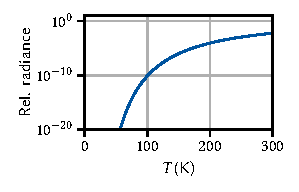
\includegraphics{img/pdf/setup/black_body_radiance}
    \caption[\imgsource{img/py/setup/cooling_power.py}]{
        Relative black-body radiance obtained by integrating \cref{eq:setup:cooling:blackbody} from \qtyrange{0}{4.5}{\micro\meter} and normalizing to the total radiance.
        At $T=\qty{300}{\kelvin}$, the fraction of total radiance residing in the high-energy part of the spectrum is still only \qty{0.6}{\percent}.
    }
    \label{fig:setup:cooling:blackbody}
\end{marginfigure}
To investigate the influence of ambient thermal radiation entering the cryostat through the optical access port, I measured the base temperature for two additional configurations; once with an additional \gls{ar}-coated window inserted into the optical path on the Cold plate, and once with three windows installed on the \gls{pt1}, \gls{pt2}, and Still plates.
The windows (\thewindow) are made from UV fused silica with \gls{ar} coating\sidenote{
    Depending on the manufacturer, the coating for the range \qtyrange{650}{1050}{\nano\meter} is called \acrshort{bbar} VIS-\acrshort{nir} or \gls{bbar}-B.
}
The manufacturer quotes a typical reflectance of \qty{0.25}{\percent} in the relevant wavelength range, while the glass is transmissive for wavelengths below $\lambda_{\mr{cutoff}}\sim\qty{4.5}{\micro\meter}$.
Since the spectral radiance of thermal black-body radiation~\cite{Planck1900}
\begin{equation}\label{eq:setup:cooling:blackbody}
    B_\lambda(\lambda, T) = \frac{2 h c^2}{\lambda^5}\frac{1}{\exp(\flatfrac{hc}{\lambda\kb T}) - 1}
\end{equation}
is small up to $\lambda_{\mr{cutoff}}$ at low ($\leq\qty{300}{\kelvin}$) temperatures as shown in \cref{fig:setup:cooling:blackbody}, we expect the windows be largely opaque to thermal radiation and hence be quite effective in reducing the radiative heat load.

\begin{margintable}
    \centering
    \footnotesize
    \caption{
        \Gls{mxc} temperature for different configurations of \gls{ar} coated windows (\thewindow) inside the \gls{dr}.
    }
    \label{tab:setup:cooling:windows}
    \begin{tabular}{lr}
        \toprule
        \textsc{Windows}                      & $T_\mathrm{\acrshort{mxc}}$ \textsc{(mK)} \\
        \midrule
        None                                  & 30.0                                      \\
        Cold                                  & 11.0                                      \\
        \acrshort{pt1}, \acrshort{pt2}, Still & 7.9                                       \\
        \bottomrule
    \end{tabular}
\end{margintable}
\begin{marginfigure}
    \centering
    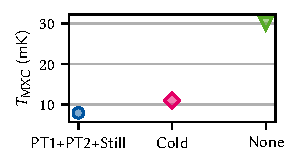
\includegraphics{img/pdf/setup/window_heating}
    \caption[\imgsource{img/py/setup/cooling_power.py}]{
        \Gls{mxc} temperature for different configurations of \gls{ar} coated windows (\thewindow) inside the \gls{dr}.
    }
    \label{fig:setup:cooling:windows}
\end{marginfigure}

\Cref{fig:setup:cooling:windows,tab:setup:cooling:windows} show the measured mixing chamber temperatures for the different window configurations.
Indeed, already a single window installed on the Cold plate significantly reduces the base temperature.
While the windows do introduce additional reflections of the laser spot when imaging the sample due to the finite remaining reflectance, their intensity is low enough, and their position on the camera far enough away from the main spot to be an issue.
On the contrary, their presence can be quite useful when aligning the laser spots from the two arms of the optical head by aligning them in such a way that the reflections overlap.

\begin{equation}\label{eq:setup:cooling:dr_power}
    P = \dot{Q} = \alpha \Tmxc^2 + \beta
\end{equation}

\begin{marginfigure}
    \centering
    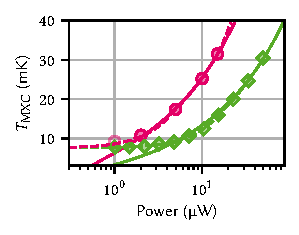
\includegraphics{img/pdf/setup/laser_heating}
    \caption[\imgsource{img/py/setup/cooling_power.py}]{
        \Acrlong{mxc} temperature as function of heater (magenta) and laser (green) power.
        Solid lines are fits to \cref{eq:setup:cooling:dr_power} including only the solid markers.
        Green dashed line is a quadratic smoothing spline fit to all laser data points.
        Magenta dashed line is the laser spline scaled to match the heater data with fitted factor $A=\qty{28}{\percent}$ corresponding to the fraction of laser power absorbed and non-radiatively emitted.
    }
    \label{fig:setup:cooling:laser}
\end{marginfigure}

\begin{marginfigure}
    \centering
    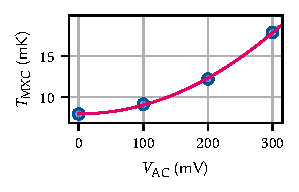
\includegraphics{img/pdf/setup/anc_readout_heating}
    \caption[\imgsource{img/py/setup/cooling_power.py}]{
        \Acrlong{mxc} temperature as function of nanopositioner AC readout voltage.
        Solid line is a fit to $T_{\mr{\acrshort{mxc}}} = a V_{\mr{AC}}^2 + b$.
        The secondary axis indicates the conversion from $T_{\mr{\acrshort{mxc}}}$ to power obtained in \cref{fig:setup:cooling:laser} which is approximately linear in this regime, leading to the expected $P\sim R\inverse V_{\mr{AC}}^2$ behavior.
        Fitting $P$ instead of $T_{\mr{\acrshort{mxc}}}$ results in $R=\qty{17.5}{\kilo\ohm}$.
        % TODO: check if V_AC is RMS or amplitude
    }
    \label{fig:setup:cooling:anc}
\end{marginfigure}

\section{Electron temperature}\label{sec:setup:cooling:etemp}
\begin{figure*}
    \centering
    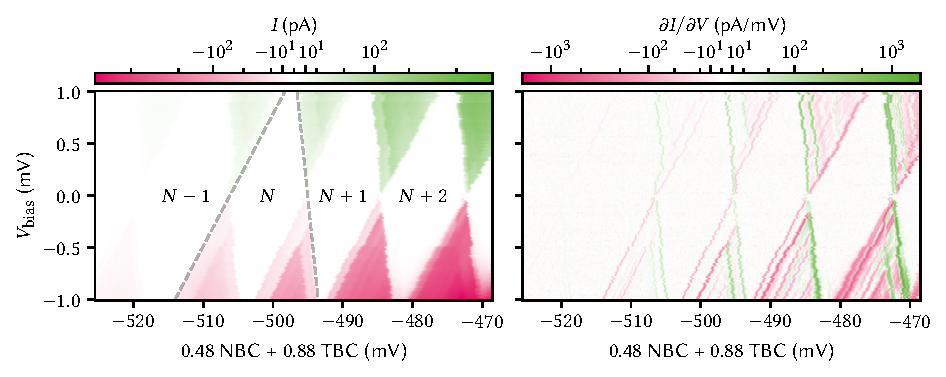
\includegraphics{img/pdf/setup/diamonds}
    \caption[\imgsource{img/py/setup/transport.py}]{}
    \label{fig:setup:cooling:etemp:diamonds}
\end{figure*}

\begin{marginfigure}
    \centering
    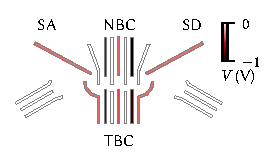
\includegraphics{img/pdf/setup/diamonds_gl}
    \caption[\imgsource{img/py/setup/transport.py}]{}
    \label{fig:setup:cooling:etemp:gl}
\end{marginfigure}

\begin{marginfigure}
    \centering
    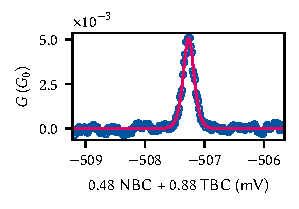
\includegraphics{img/pdf/setup/coulomb_resonance}
    \caption[\imgsource{img/py/setup/transport.py}]{}
    \label{fig:setup:cooling:etemp:resonance}
\end{marginfigure}
